\section{邻接与路径}
\label{sec:graph-adjacency-paths}

贯穿图\eqref{eq:graph-conn-running-graph}中顶点$1$和$4$之间没有边，却可以先到$2$或$3$，再到$4$。“一步能到谁”由边集直接读出；“若干步能到谁”则要把边首尾相接。本节先描述一个顶点的直接邻居，再定义多步的行走和路径，区分无向环与有向环，最后建立可达关系。边上若有长度，怎样比较不同路线的总成本是第~\ref{sec:graph-shortest-paths}节的问题，这里只讨论哪些顶点序列允许通行。

\subsection{邻接、邻域与度}
\label{sec:graph-conn-neighborhoods}

在无向图中，若$\{i,j\}\in E$，称$i$与$j$\term{邻接}（adjacent），互为邻居。顶点$i$的全部邻居组成它的\term{邻域}（neighborhood）
\[
N(i)=\{j\in V:\{i,j\}\in E\},
\]
邻居的个数$d_i=|N(i)|$称为$i$的\term{度}（degree）。贯穿图中$N(1)=\{2,3\}$，$N(2)=\{1,3,4\}$，四个顶点的度依次为$2,3,3,2$。度只数直接邻居；$1$经过两步可以到达$4$，但$4$不计入$N(1)$。

\paragraph{有向图的两种邻域}
在有向图中，一条弧$i\to j$对两个端点的意义不同：对$i$来说$j$是下一步可以到达的顶点，对$j$来说$i$是能一步到达它的顶点。因此要分别定义出邻域与入邻域：
\[
N^+(i)=\{j:(i,j)\in E\},\qquad
N^-(i)=\{j:(j,i)\in E\}.
\]
二者的大小$d_i^+=|N^+(i)|$与$d_i^-=|N^-(i)|$分别称为\term{出度}（out-degree）与\term{入度}（in-degree）。以图~\ref{fig:graph-conn-direction-orientation}(e)的$1\to2\leftarrow3$为例，$N^-(2)=\{1,3\}$，$N^+(2)=\varnothing$：两个顶点能一步到达$2$，从$2$出发却一步也走不了。报告“$2$的邻居”时若不说明方向，就可能把入邻居误当成下一步可以到达的顶点。

\paragraph{度数和与边数}
把每个顶点的度加起来，会得到一个只与边数有关的量。考虑所有“顶点—边”配对$(i,e)$，其中$i$是边$e$的端点。按顶点分组，顶点$i$出现在$d_i$个配对中；按边分组，每条边恰有两个端点，出现在两个配对中。两种分组数的是同一批配对，所以
\begin{equation}
\sum_{i\in V}d_i=2m.
\label{eq:graph-conn-handshake}
\end{equation}
贯穿图中$2+3+3+2=10=2\times5$。由此还可知，度为奇数的顶点个数必是偶数，否则左边为奇数。在有向图中，每条弧恰好贡献一个出度和一个入度，同样的分组给出
\[
\sum_{i\in V}d_i^+=\sum_{i\in V}d_i^-=m;
\]
例如图~\ref{fig:graph-conn-direction-orientation}(d)的$1\to2\to3$中，出度为$1,1,0$，入度为$0,1,1$，两组之和都是弧数$2$。这里的度只数结构上的边，不涉及边权；把邻边权重累加起来的加权度在第~\ref{sec:graph-vertex-edge-functions}节另行定义。

\subsection{行走、路径与环}
\label{sec:graph-conn-walks-paths}

把相邻的边首尾相接，就得到一串顶点。是否允许重复经过同一个顶点，会得到用途不同的对象：反复传播、来回巡视的过程允许重复，一条实际路线通常不允许。

\begin{definition}[行走与路径]
\label{def:graph-conn-walk-path}
设$\mathcal G=(V,E)$是无向图。顶点序列$(v_0,\ldots,v_k)$若对每个$r=1,\ldots,k$都有$\{v_{r-1},v_r\}\in E$，就称为从$v_0$到$v_k$的一条\term{行走}（walk），$k$称为它的长度，即经过的边数。若行走中的顶点两两不同，就称为一条简单\term{路径}（path）。
\end{definition}

行走允许重复经过顶点和边；单个顶点$(v_0)$是长度为零的行走，也是长度为零的路径。本部分不加修饰的“路径”都指简单路径。图~\ref{fig:graph-conn-walk-path-cycle}(a)的$(1,2,3,1,2)$是长度为$4$的行走，它两次经过边$\{1,2\}$；(b)的$(1,2,4)$是长度为$2$的路径。

\begin{figure}[!htb]
  \centering
  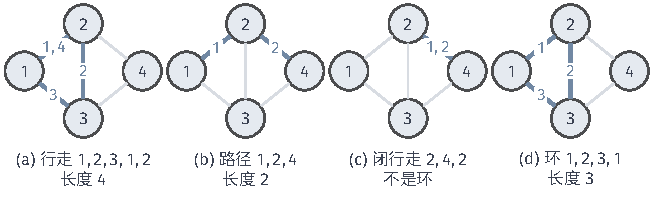
\includegraphics[width=110.688mm]{figures/01-basic-mathematics/04-graphs/tikz/c1-walk-path-cycle/figure.pdf}
  \caption{贯穿图上的四种顶点序列。蓝色粗线是经过的边，边旁数字是经过该边的步序，浅灰色是未经过的边。(a)行走可以重复经过边$\{1,2\}$；(b)路径不重复顶点；(c)沿一条边去而复返得到闭行走，但它不是环；(d)绕三角形一周的环除首尾外不重复顶点。}
  \label{fig:graph-conn-walk-path-cycle}
\end{figure}

\paragraph{闭行走与环}
首尾相同（$v_0=v_k$）的行走称为\term{闭行走}（closed walk）。闭合并不意味着绕成了一圈：图~\ref{fig:graph-conn-walk-path-cycle}(c)的$(2,4,2)$沿边$\{2,4\}$去而复返，是长度为$2$的闭行走，却没有围出任何区域。为了排除这种情形，把长度$k\geq3$、且$v_0,v_1,\ldots,v_{k-1}$两两不同的闭行走称为\term{环}（cycle）。长度下限来自简单图的约定：长度为$1$的闭行走需要自环，长度为$2$的闭行走$(v_0,v_1,v_0)$只能沿同一条边往返。图~\ref{fig:graph-conn-walk-path-cycle}(d)的$(1,2,3,1)$是长度为$3$的环。

同一个环可以从不同顶点出发、沿两个方向书写，例如$(1,2,3,1)$、$(2,3,1,2)$和$(1,3,2,1)$经过的是同一组边。计数环或比较两个环时，我们把经过同一组边的序列看成同一个环。

\subsection{有向路径与有向无环图}
\label{sec:graph-conn-dag}

任务依赖要求每一步都顺着箭头走：从任务$i$出发，只能走到依赖$i$的任务。把定义~\ref{def:graph-conn-walk-path}中的条件$\{v_{r-1},v_r\}\in E$换成$(v_{r-1},v_r)\in E$，就得到有向行走与\term{有向路径}（directed path）；长度、闭合与顶点不重复的含义不变。

\paragraph{有向环}
除首尾外顶点两两不同、长度至少为$1$的有向闭行走称为\term{有向环}（directed cycle）。由于排除了自环，有向环的长度至少为$2$；与无向情形不同，长度为$2$的有向环是允许的。图~\ref{fig:graph-conn-directed-cycle-dag}(a)中两条反向弧$i\to j$和$j\to i$是两个不同的对象，$(i,j,i)$依次经过它们，构成一个有向环；而无向图中的$(2,4,2)$两次经过的是同一条边。图~\ref{fig:graph-conn-directed-cycle-dag}(b)的$(1,2,3,1)$每一步都顺着箭头，是长度为$3$的有向环。

\begin{figure}[!htb]
  \centering
  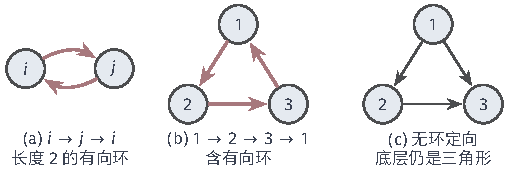
\includegraphics[width=85.937mm]{figures/01-basic-mathematics/04-graphs/tikz/c1-directed-cycle-dag/figure.pdf}
  \caption{有向环与有向无环图。红色弧组成有向环。(a)两条反向弧构成长度为$2$的有向环；(b)三角形的循环定向含有向环；(c)同一个三角形的另一种定向不含有向环，是有向无环图，尽管它的底层无向图是一个环。}
  \label{fig:graph-conn-directed-cycle-dag}
\end{figure}

\paragraph{有向无环图}
如果任务之间的依赖形成有向环，例如$1$等$2$、$2$等$3$、$3$又等$1$，这组任务就无法按任何次序全部完成。不含有向环的依赖才可能排出顺序。

\begin{definition}[有向无环图]
\label{def:graph-conn-dag}
不含有向环的有向图称为\term{有向无环图}（directed acyclic graph，DAG）。
\end{definition}

“无环”只针对有向环。图~\ref{fig:graph-conn-directed-cycle-dag}(c)的弧为$1\to2$、$1\to3$、$2\to3$，逐个检查长度为$2$和$3$的闭合序列，没有一个能每步都顺着箭头：例如$(1,2,3,1)$的最后一步需要弧$3\to1$，而图中只有$1\to3$。所以它是DAG，但去掉箭头后得到一个三角形，底层无向图是有环的。第~\ref{sec:graph-topological-order}节的拓扑排序要求的正是有向无环，不能换成“底层无向图无环”这个更强的条件。

\subsection{可达性}
\label{sec:graph-conn-reachability}

前面的定义描述的是具体的顶点序列。很多问题只关心“能不能到”，而不关心怎么到。

\paragraph{可达关系}
若存在从$i$到$j$的行走，称$j$从$i$\term{可达}（reachable）；有向图中要求有向行走。行走允许重复顶点，使用起来比路径方便：从$i$到$j$的行走接上从$j$到$k$的行走，仍是一条行走，而两条路径首尾相接后可能重复经过顶点。下面的引理说明，判断可达时用行走还是路径并没有区别。

\begin{lemma}[行走中含有路径]
\label{lem:graph-conn-walk-contains-path}
在无向图或有向图中，若存在从$i$到$j$的行走，则存在从$i$到$j$的路径，并且它的顶点和边都取自这条行走。
\end{lemma}

\begin{proof}
在从$i$到$j$、顶点和边都取自原行走的所有行走中，取长度最短的一条$(v_0,\ldots,v_k)$。若它不是路径，则有$s<t$使$v_s=v_t$。删去中间段$v_{s+1},\ldots,v_t$，得到$(v_0,\ldots,v_s,v_{t+1},\ldots,v_k)$：原来从$v_t$出发的那一步现在从$v_s=v_t$出发，因此每一步仍沿原有的边或弧，而长度减少了$t-s>0$，与长度最短矛盾。所以最短的那条行走就是路径。
\end{proof}

由定义和引理，可达关系有以下性质。零长度行走使每个顶点从自身可达，即自反性；行走首尾相接说明传递性；在无向图中把行走倒过来走仍是行走，所以还有对称性。因此无向图上的可达关系是第~\ref{sec:prelim-equivalence-relations}节意义下的等价关系，下一节将据此划分连通分量。

\paragraph{有向图中可达不对称}
有向图中倒过来走需要反向弧，对称性一般不成立。在图~\ref{fig:graph-conn-direction-orientation}(d)的单向链$1\to2\to3$中，$3$从$1$可达，$1$却不从$3$可达。为了描述这种单向的关系，把一步关系与多步关系分别命名：$N^-(j)$中的顶点称为$j$的直接\term{前驱}（predecessor），$N^+(j)$中的顶点称为直接\term{后继}（successor）；能经过一条或多条弧到达$j$的其他顶点称为$j$的\term{祖先}（ancestor），从$j$出发经过一条或多条弧能到达的其他顶点称为$j$的\term{后代}（descendant）。本部分约定祖先与后代都不含$j$自身。

在单向链中，$3$的直接前驱只有$2$，祖先则是$\{1,2\}$；$1$的后代是$\{2,3\}$，$3$没有后代。有向环上的两个不同顶点可以互为祖先，例如图~\ref{fig:graph-conn-directed-cycle-dag}(b)中的$1$和$2$；在DAG中这不可能发生。若$i\neq j$互为祖先，把$i$到$j$与$j$到$i$的两条有向路径拼起来，得到一条长度至少为$2$的有向闭行走$(v_0,\ldots,v_k)$，其中$v_0=v_k$。在所有满足$s<t$、$v_s=v_t$的位置对中取$t-s$最小的一对，则$(v_s,\ldots,v_t)$除首尾外不重复顶点；它的长度不能为$1$（没有自环），所以是一个有向环，与DAG的定义矛盾。可达的不对称性使有向图的“连通”需要两种不同的定义，这是下一节的内容。
